\documentclass{article}

% if you need to pass options to natbib, use, e.g.:
%     \PassOptionsToPackage{numbers, compress}{natbib}
% before loading neurips_2019

% ready for submission
% \usepackage{neurips_2019}

% to compile a preprint version, e.g., for submission to arXiv, add add the
% [preprint] option:
%     \usepackage[preprint]{neurips_2019}

% to compile a camera-ready version, add the [final] option, e.g.:
\usepackage[]{neurips_2019}

% to avoid loading the natbib package, add option nonatbib:
%     \usepackage[nonatbib]{neurips_2019}

\usepackage[utf8]{inputenc} % allow utf-8 input
\usepackage[T1]{fontenc}    % use 8-bit T1 fonts
\usepackage{hyperref}       % hyperlinks
\usepackage{url}            % simple URL typesetting
\usepackage{booktabs}       % professional-quality tables
\usepackage{amsfonts}       % blackboard math symbols
\usepackage{nicefrac}       % compact symbols for 1/2, etc.
\usepackage{microtype}      % microtypography
\usepackage{graphicx}
\graphicspath{{./images/}}

\title{Math189 Midterm Report: Instrument Recognition Through Machine Learning}

\begin{document}

\maketitle

\begin{abstract}
  Automated instrument recognition a desirable task within the The music information retrieval (MIR) field. Although humans are relatively adept at distinguishing between instruments, a robust Artificial intelligence system would provide valuable application purposes. This project will demonstrate how both shallow and deep Machine learning algorithms can be used to identify the instrument being played in a monophonic audio track.
\end{abstract}

\section{Introduction}

Music is most often created through a combination of instruments and vocals. With adequate exposure, a human can usually identify common instruments that are used in a music; However, due to stylistic differences between artists and the quality differences between recordings, it is still difficult for computers automatically recognize individual instruments.

In the current digitized world, music is highly accessible through the internet and various streaming platforms. The high availability of recordings makes instrument recognition a desirable task within the The music information retrieval (MIR) field. The ability to automate instrument recognition will allow for processes commonly used in music related platforms, such as genre classification and song recommendation, to be improved.

The goal of this project is to create and compare machine learning models that can identify the instrument being played in a monophonic audio track. To narrow the scope of this project, the model has been limited to the classification of 10 musical instruments: bass, brass, flute, guitar, keyboard, mallet, organ, reed, string, vocal. While deep learning techniques are often used in instrument recognition[1], this project will cover both shallow and deep learning approaches and compare their effectiveness.

\section{Dataset}
\label{Dataset}

The dataset being used by this project is called the Nsynth Dataset provided by Magenta, an open source Python library. NSynth contains 305,979 musical notes with each audio file having a unique pitch, timbre, and envelope. These samples are annotated based on a both human evaluation and heuristic algorithms and contains information on the following:

\begin{itemize}
\item Source: Contains be labeled acoustic, electronic, or synthetic based on the method of sound production for the audio clip. Each note is labeled with a single source.
\item Family: Contain the labels bass, brass, flute, guitar, keyboard, mallet, organ, reed, string, synth lead, vocal. This indicated the high-level family of the instrument being played and each note is labeled with a single family. 
\item Qualities: Contains the labels bright, dark, distortion, fast decay, long release, multiphonic, nonlinear env, percussive, reverb, and tempo-synced. These labels are given based on the sonic qualities of the note and each note is annotated with zero or more qualities.
\end{itemize}

For the purposes of this model, the "family" of each note is used to determine the instrument.

The dataset is split into three sets: train, test, and validation.An example of the data distribution of a dataset is shown in figure 1. Due to the imbalance of data according to instrument family, under-sampling was implemented to ensure an equal number of samples in each family. Note that due to ambiguity of the label meaning, all samples classified as synth lead was later dropped from the dataset. The resulting number of samples is used recorded in table 1.

\begin{figure}[htb]
  \centering
  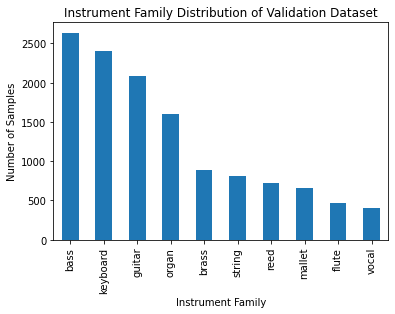
\includegraphics[width=.35\linewidth]{validation_distribution}
  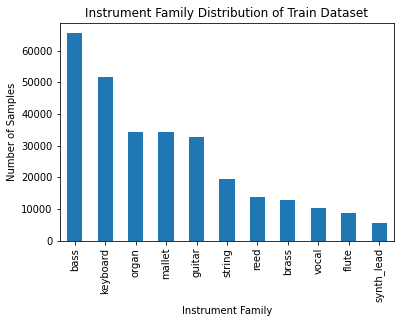
\includegraphics[width=.35\linewidth]{train_distribution}
  \caption{Train and Validation Data Set Distributions}
\end{figure}
\begin{table}[htb]
  \caption{Nsynth Dataset Breakdown}
  \label{Nsynth-Dataset}
  \centering
  \begin{tabular}{llc}
    \toprule
    Set name & Samples & Samples Used (After Under-sampling)\\
    \midrule
    Train & 289,205 & 55,000\\
    Test & 12,678 & 4,000\\
    Validation & 4,096 & N/A\\
    \bottomrule
  \end{tabular}
\end{table}


\section{Audio Features}
\label{features}

In order to better represent the musical samples as data points for the model, various features where extracted and used from each sample rather than the raw audio.

\subsection{Features}
The following features were selected for consideration based on a literature review[2][3]:
\begin{itemize}
    \item \textbf{Chroma}: The chroma of a signal is extracted by casting an audio signal into 12 semitones (chromas) based on their pitch within the musical octave. These features loses information regarding the absolute frequency of the signal but is useful in identifying relation between chroma of the audio signal.
    \item \textbf{Harmonic/Percussive}: Harmonic sounds are perceived as pitched sound (eg. melodies, chords) where as percussive sound are noise-like and usually stems from instrument onsets (eg. hit on a drum, consonants in speech). The Harmonic/Percussive feature uses the ratio of harmonic to percussive sounds to classify whether the sound is more harmonic or more percussive.
    \item \textbf{Mel-Frequency Cepstral Coefficient (MFCC}: The Mel-Frequency Cepstrum is found by spacing the frequency bands of the spectrum of a signal equally along the mel scale, and then taking the Fourier transform of the logarithm of the spectrum. The coefficients of this transformation represent the power spectrum of the signal
    \item \textbf{Mel Spectrogram}: A spectrogram is an intensity plot of the Short-Time Fourier Transform (STFT) magnitude. The spectrogram used for the model was adjusted to the mel scale, which represents pitches judged by listeners to be equal in distance one from another.
    \item \textbf{Spectral Centroid}: Spectral centroid is determined by the mean of each frame in the spectrogram after its magnitude has been normalized.
    \item \textbf{Spectral Contrast}: Spectral contrast is a measure of the difference in the spectral peak and the spectral valley in each frequency sub-band.
    \item \textbf{Spectral Rolloff}: The spectral roll-off is determined by the frequency at each frame below which ${85}\%$  of the energy in the spectrogram is contained. The feature is used to differentiate sounds with different energy distributions.
    \item \textbf{Zero-Cross Rating}: The Zero-Cross rate is determined by the rate of sign-changes in an audio time series. The rate is found to be higher for noisy audio and audio that includes higher frequency signals.
\end{itemize}

\subsection{Feature Evaluation}

In order to evaluate each feature independently, a random forest model using was implemented using each feature exclusively. For this process, the Validation dataset with a test size of 0.1 was used. Confusion matrices from the resulting models are shown in figure 2. 

\begin{figure}[htb]
  \centering
  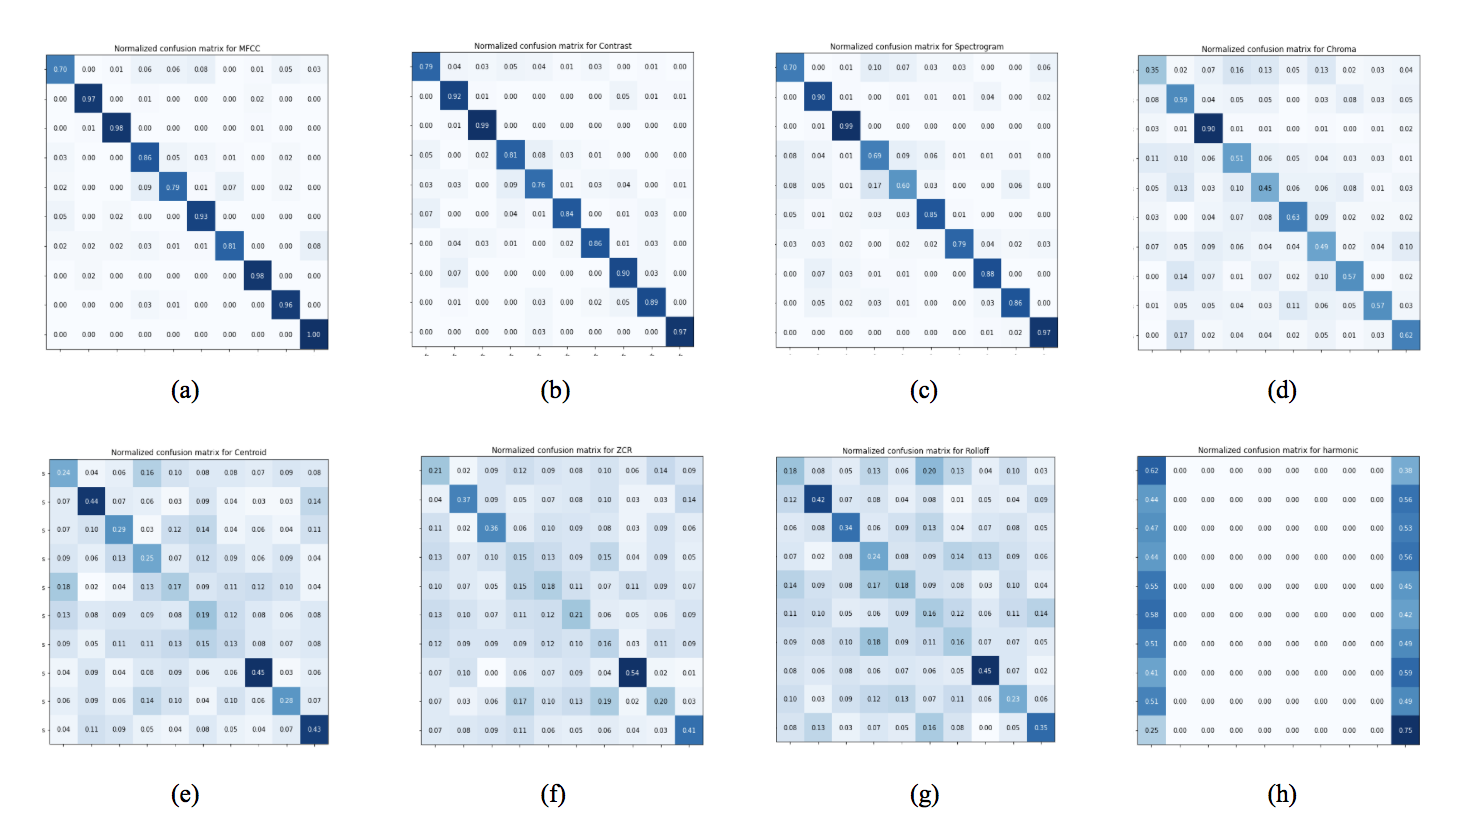
\includegraphics[width=1\linewidth]{cm_feat}
  \caption{Feature Models Confusion Matrices for (a) MFCC (b) Spectral Contrast (c) Spectrogram (d) Chroma (e) Spectral Centroid (f) ZCR (g) Spectral Rolloff (h) harmonic/percussive }
\end{figure}

From these results, the accuracy of each feature model was used as a metric for the associated feature's importance. Thus, the ordering of feature importance is shown in table 2.

\begin{table}[htb]
  \caption{Features and Accuracy}
  \label{Nsynth-Dataset}
  \centering
  \begin{tabular}{ll}
    \toprule
    Model feature & Accuracy(\%) \\
    \midrule
    Mfcc & 89.90 \\
    Spectral Contrast & 87.30\\
    Spectrogram & 82.30\\
    Chroma & 56.80\\
    Spectral Centroid & 28.70\\
    Zero-cross Rating & 27.90\\
    Spectral Rolloff & 27.10\\
    Harmonic/Percussive & 13.70\\
    \bottomrule
  \end{tabular}
\end{table}

Since there are 10 labels in these models a random selection should yield an accuracy rate of 20\%, therefore all of the features evaluated except the  Harmonic/Percussive feature has some measure of discriminatory ability. By using all features excluding the Harmonic/Percussive feature, model of 93.90\% can be implemented, as shown in figure 3. Keep in mind that, due to the randomized nature of the train test split process when implementing the Random Forest Model, the accuracy of the models may fluctuate up to $\pm 1.00\%$.

\begin{figure}[htb]
  \centering
  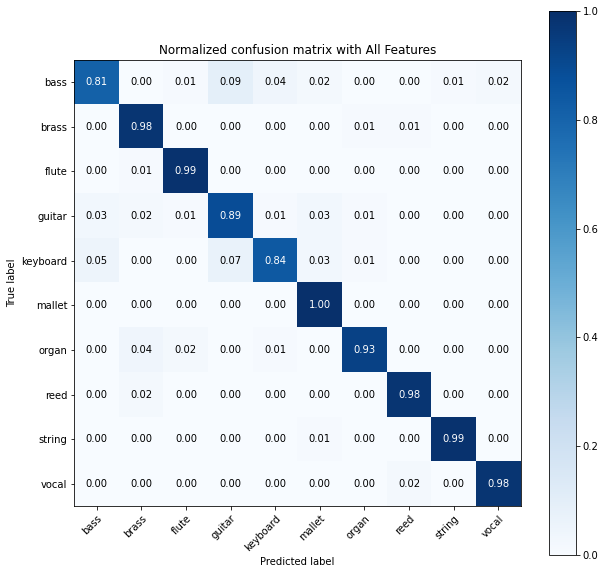
\includegraphics[width=.5\linewidth]{cm_all_feat}
  \caption{Confusion Matrix for Model without Harmonic/Percussive Feature}
\end{figure}

Although using all features except for the Harmonic/Percussive feature shows promising results, in order to optimize the feature extraction process, features that contribute relatively insignificantly are also excluded from the process. Starting with the worst performing features, each feature is discarded from the input data until the model is shown to be affected. When discarding all features up through Chroma features(figure 4 (a)) the model output accuracy was 93.70\%, which is within the original output of 93.90\%$\pm 1.00\%$. However when the Spectrogram feature was also discarded(figure 4 (a)), the accuracy decreased to 91.20\%. 

\begin{figure}[htb]
  \centering
  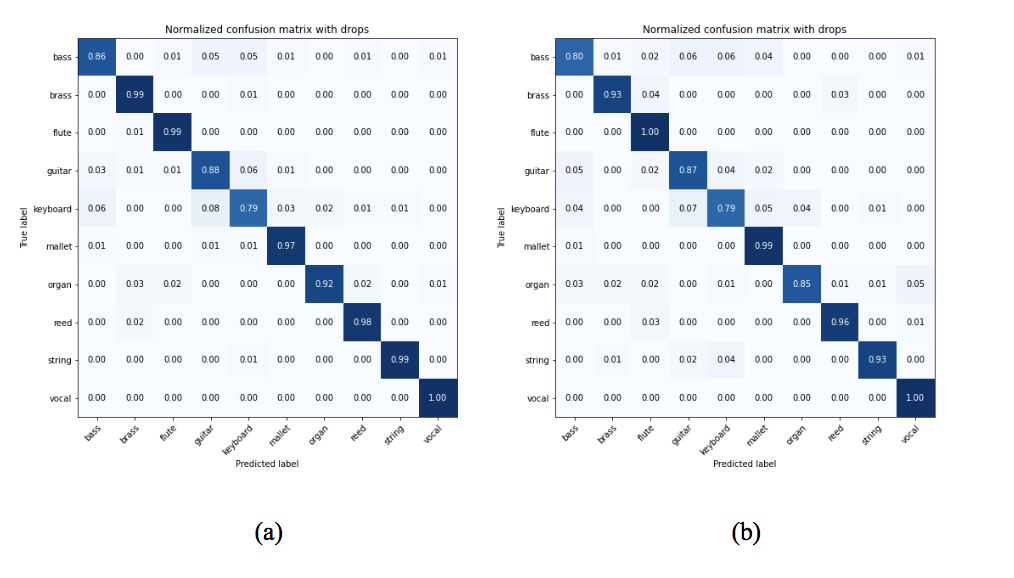
\includegraphics[width=1\linewidth]{cm_drop}
  \caption{Confusion Matrix for Model (a) with MFCC, Contrast, and Spectrogram (b) with MFCC and Contrast}
\end{figure}

Ultimately, the MFCC, Contrast, and Spectrogram features were used as data input for the final models.

\section{Random Forest Model}

In order to train the instrument recognition model, a few different machine learning models where implemented, including: Random forest, Support-vector machine(SVM), Bayesian, and Principal Component analysis. SVMs have commonly been used in instrument recognition applications [4]; however, from initial results, the accuracy of the Random forest algorithm outperformed all other models, and therefore it was used as the final model architecture. 

\subsection{Results}
For the final Random Forest model, the Train dataset was used with a test size of 0.1. The results of the Random forest model is used to generate the normalized confusion matrix in figure 5.

\begin{figure}[htb]
  \centering
  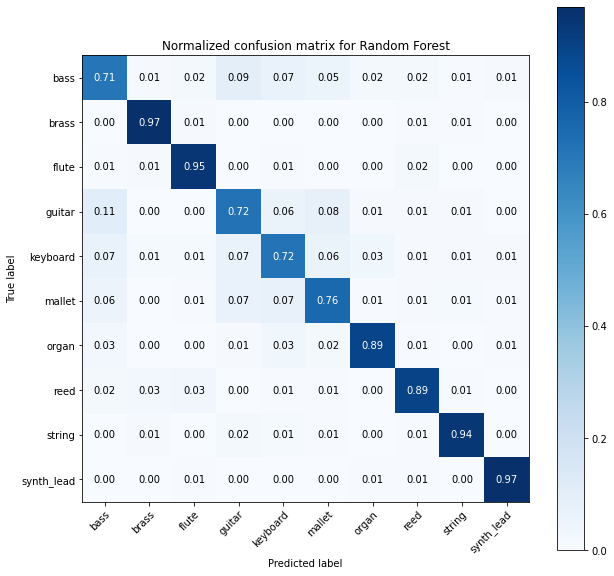
\includegraphics[width=.6\linewidth]{confusion_matrix}
  \caption{Output of the Random Forest Model}
\end{figure}

This confusion matrix illustrates a relatively high performance across all types of instrument recognition, a further breakdown of the results are detailed in table 2. 

\begin{table}[htb]
  \caption{Model Results Breakdown (Ordered by Descending Accuracy)}
  \label{results-table}
  \centering
  \begin{tabular}{ccccc}
    \toprule
    Instrument & accuracy & precision & recall & f1-score  \\
    \midrule
    vocal & 0.97 & 0.96 & 1.97 & 0.96\\
    brass & 0.97 & 0.92 & 0.97 & 0.95\\
    flute & 0.95 & 0.91 & 0.95 & 0.93\\
    string & 0.94 & 0.94 & 0.94 & 0.94\\
    organ & 0.89 & 0.92 & 0.89 & 0.91\\
    reed & 0.89 & 0.91 & 0.89 & 0.90\\
    mallet & 0.76 & 0.77 & 0.76 & 0.76\\
    guitar & 0.72 & 0.73 & 0.72 & 0.73\\
    keyboard & 0.72 & 0.73 & 0.72 & 0.72\\
    bass & 0.71 & 0.72 & 0.71 & 0.71\\
    \bottomrule
  \end{tabular}
\end{table}

These results show an accuracy range of $71.00\%-97.00\%$ and a f1-score range of $71.00\%-96.00\%$, which the accuracy being a relative predictor for f1-score performance. The overall accuracy of the model comes out to be $85.16\%$.



\section{Long Short-Term Memory Model}

Since Long Short Term Memory networks (LSTMs) are capable of learning long-term dependencies, they were used in the deep learning instrument recognition model. The overall architecture of the model utilized two LSTM layers as well as two Density Layers with different activations (relu and softmax). An overview of the Neural Network layers are illustrated in figure 6.

\begin{figure}[htb]
  \centering
  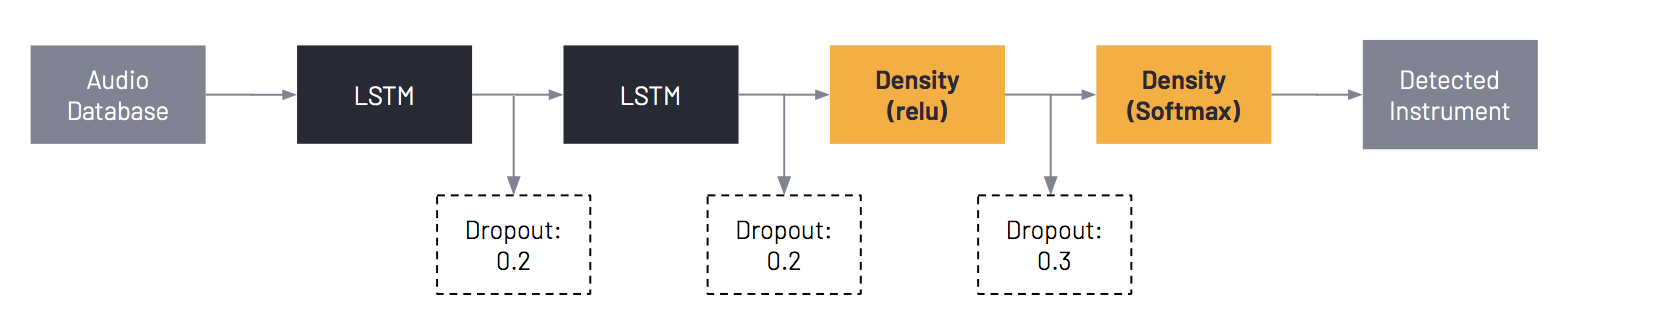
\includegraphics[width=1.1\linewidth]{architecture}
  \caption{Deep Learning Model Setup}
\end{figure}

Although audio deep learning networks often intake raw audio or spectrograms rather than specific features, in order to ensure fair comparison, between models, identical datapoints from the Random Forest Model were also used to inform the LSTM model.

\subsection{Results}
For the final LSTM model, the Train dataset was used with a test size of test size of 0.1, validation size of 0.9, batch size of 32, and 75 epochs.  The results of the LSTM model is used to generate the normalized confusion matrix in figure 7.

\begin{figure}[htb]
  \centering
  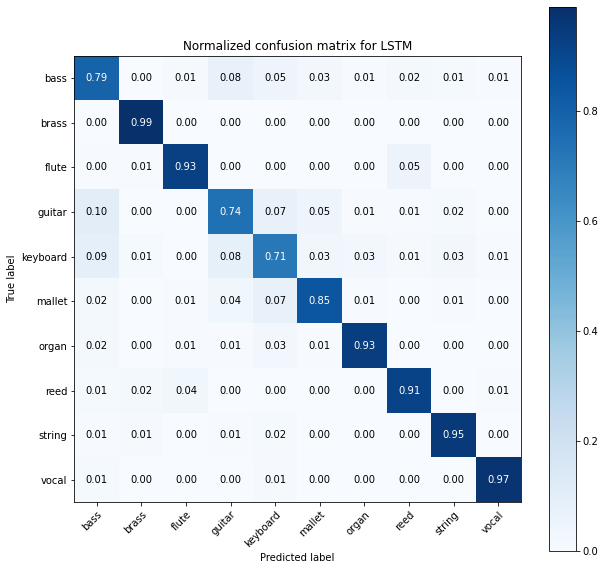
\includegraphics[width=.6\linewidth]{cm_lstm}
  \caption{Output of the LSTM Model}
\end{figure}

This confusion matrix illustrates a relatively high performance across all types of instrument recognition, a further breakdown of the results are detailed in table 2. 

\begin{table}[htb]
  \caption{Model Results Breakdown (Ordered by Descending Accuracy)}
  \label{results-table}
  \centering
  \begin{tabular}{ccccc}
    \toprule
    Instrument & accuracy & precision & recall & f1-score  \\
    \midrule
    brass & 0.99 & 0.94 & 0.99 & 0.96\\
    vocal & 0.97 & 0.97 & 1.97 & 0.97\\
    string & 0.95 & 0.93 & 0.95 & 0.94\\
    flute & 0.93 & 0.94 & 0.93 & 0.93\\
    organ & 0.93 & 0.95 & 0.93 & 0.94\\
    reed & 0.91 & 0.90 & 0.91 & 0.91\\
    mallet & 0.85 & 0.87 & 0.85 & 0.86\\
    bass & 0.79 & 0.74 & 0.79 & 0.77\\
    guitar & 0.74 & 0.79 & 0.74 & 0.74\\
    keyboard & 0.71 & 0.74 & 0.71 & 0.73\\
    \bottomrule
  \end{tabular}
\end{table}

These results show an accuracy range of $71.00\%-99.00\%$ and a f1-score range of $73.00\%-96.00\%$, which the accuracy being a relative predictor for f1-score performance. The overall accuracy of the model comes out to be  $87.73\%$.


\section{Discussion}

\subsection{Error Analysis}

An interesting point to observe is that the optimal model produced during the feature evaluation process, which used the validation dataset, had an accuracy of 93.90\% while the final model, which uses the train dataset, had an accuracy of 85.16\%. This outcome is unexpected since the train dataset has significantly more audio samples than the validation set. However, there are some factors such as, source type, that vary between the datasets. The proportion of synthetic samples in the train dataset is larger than the validation dataset.

By dropping all synthetic samples from the train dataset and balancing the it, the dataset retains only samples produced by electronic and acoustic sources with a the distribution shown in figure 8. After balancing, 3960 samples of each instrument were used for training and testing.

\begin{figure}[htb]
  \centering
  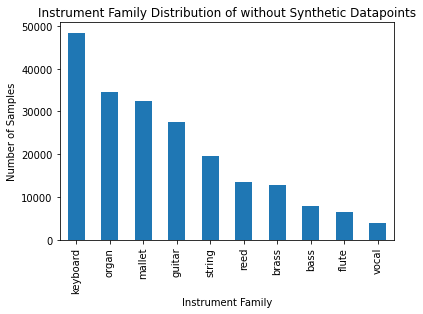
\includegraphics[width=.5\linewidth]{nonsynth_distribution}
  \caption{Train Data Set without Synthetic Sources Distribution}
\end{figure}

By running the Random Forest model on this modified dataset, the model has an 88.18\% accuracy and the confusion matrix shown in figure 9.

\begin{figure}[htb]
  \centering
  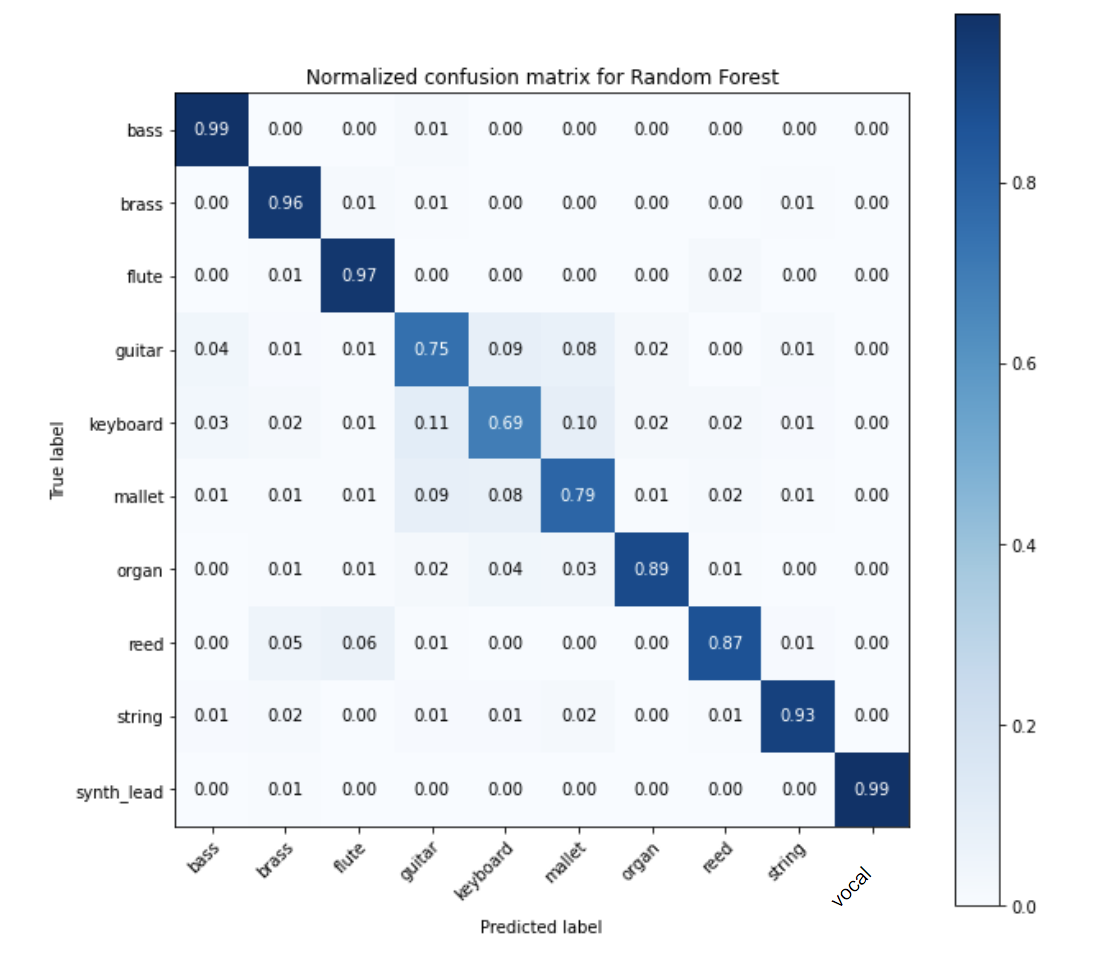
\includegraphics[width=.6\linewidth]{cm_nonsynth}
  \caption{Confusion Matrix for Model without Synthetic Sources}
\end{figure}

By dropping the synthetic samples, the overall performance of the model increased by about 3\%. The accuracy of recognizing the bass, which had the overall highest number and proportion of synthetic samples, increased from 71.00\% to 99.00\%, while other instruments with less synthetic samples all changed in accuracy by $\pm5.00\%$. These changes suggest that the source of the samples have a nontrivial influence on the accuracy of the model, and that some synthetic instruments samples are particularly difficult to classify.

Aside from the type of source, the unique instrument that a sample comes from may also affect the model results. Since the train dataset is much larger, the samples within the train dataset come from 953 unique instruments as opposed to the 53 unique instruments that the validation dataset comes from. Therefore, the model output may decrease in accuracy as number of instruments increase since each instrument will have have a slightly different intonations and may fundamentally differ in audio signatures.

In addition to factors caused by the samples themselves, there are some instruments that the model is specifically poor at distinguishing between; for example, $8.00\%$ of the guitar samples are incorrectly classified as mallet while $7.00\%$ of the mallet samples are incorrectly classified as guitar, therefore suggesting that mallet and bass are particularly similar in terms of features. Examples of mislabelling are highlighted in figure 9.

\begin{figure}[htb]
  \centering
  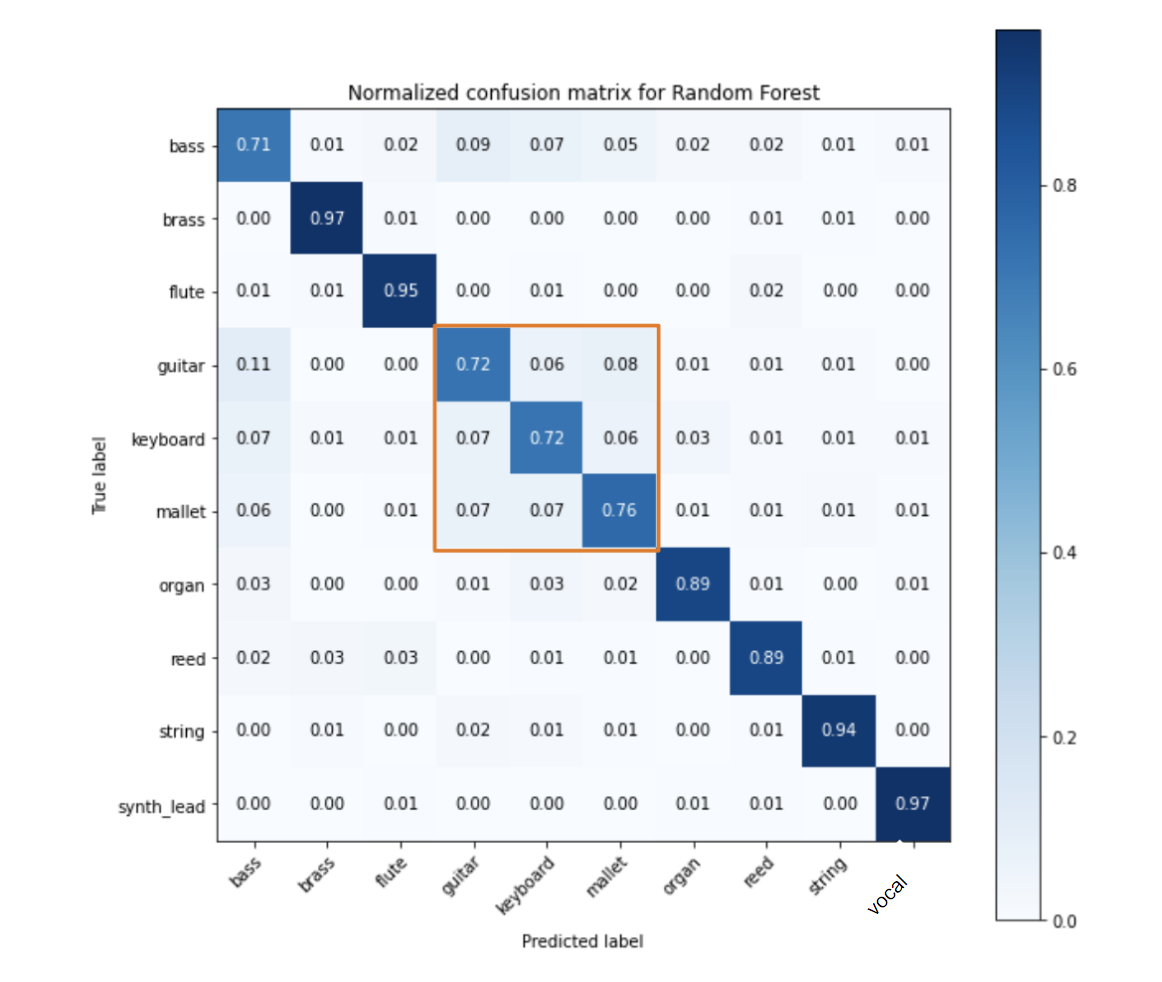
\includegraphics[width=.6\linewidth]{mislabel}
  \caption{Areas of Common Mislabeling}
\end{figure}

\subsection{Conclusion}

From the accuracy and f1-scores of the Random Forest and LSTM models, the overall performance of both models seems fairly good and similar to one another. While the final LSTM model outperformed the Random Forest Model by a small margin $(~2.00\%)$, this difference is not extremely big, especially since the Forest Model fluctuates in accuracy $\pm1.00\%$ depending on the train test split. Furthermore, the Random Forest model had marginally outperformed the LSTM model in initial results when using smaller data sets. Thus, there is no clear distinction on whether a shallow or deep learning approach is more optimal in instrument recognition. Rather, the best architecture likely depends on available data, computation power, and run-time constraints.

\subsubsection*{Acknowledgments}

I would like to thank Prof. Gu and Siddarth for their support and
feedback throughout the the project development
process.

\section*{References}

[1] Mazarakis, Giorgos & Tzevelekos, Panagiotis & Kouroupetroglou, Georgios. (2006). Musical Instrument Recognition and Classification Using Time Encoded Signal Processing and Fast Artificial Neural Networks. 246-255. 10.1007/11752912\_26. 

[2] Kim, Daeyeol & Sung, Tegg & Cho, S. & Lee, Gyunghak & Sohn, Chae. (2018). A Single Predominant Instrument Recognition of Polyphonic Music Using CNN-based Timbre Analysis. International Journal of Engineering and Technology(UAE). 7. 590-593. 10.14419/ijet.v7i3.34.19388. 

[3] Sigtia, Siddharth & Benetos, Emmanouil & Dixon, Simon. (2015). An End-to-End Neural Network for Polyphonic Music Transcription. IEEE/ACM Transactions on Audio, Speech, and Language Processing. 24. 10.1109/TASLP.2016.2533858. 

[4] Prabhjyot Singh1, Dnyaneshwar Bachhav2, Omkar Joshi3, Nita Patil4. Singh, Prabhjyot & Bachhav, Dnyaneshwar & Joshi, Omkar & Patil, Nita. (2019). Musical Instrument Recognition using CNN and SVM. IRJET. 6. 3. 

\end{document}

